\documentclass[11pt,a4paper]{article}

% --- Encoding & Language ---
\usepackage[T1]{fontenc}
\usepackage[utf8]{inputenc}
\usepackage[swedish]{babel}

% --- Math ---
\usepackage{amsmath,amssymb}

% --- Layout ---
\usepackage[a4paper,margin=2.5cm]{geometry}
\usepackage{microtype}

% --- Lists ---
\usepackage{enumitem}

% --- Table of contents formatting ---
\usepackage{tocloft}

% --- Hyperlinks ---
\usepackage[hidelinks]{hyperref}

% --- Code ---
\usepackage{listings}
\usepackage{xcolor}

% --- images ---
\usepackage{graphicx}
\graphicspath{{images/}}

\lstdefinestyle{pseudocode}{
  basicstyle=\ttfamily\small,
  columns=fullflexible,
  frame=single,
  breaklines=true,
  numbers=none,
  showstringspaces=false,
  tabsize=2,
  breakatwhitespace=false
}

\title{
\vspace{3cm}
\Huge \textbf{Fysikalisk Modell för 2D-Simulering av Ljud} \\
\vspace{0.5cm}
\Large Interaktiv installation för Tom Tits
}

\author{Leo Ehrenberg}
\date{15/03/26}

\begin{document}

\maketitle
\thispagestyle{empty}

\vspace{2cm}

\begin{center}
\begin{minipage}{0.85\textwidth}
\section*{Introduktion}

Detta dokument beskriver den fullständiga fysikaliska grund som används för att
simulera ljudutbredning i ett tvådimensionellt plan. Modellen är framtagen
för en interaktiv installation där barn visuellt kan observera hur ljud
sprids, reflekteras och interagerar med olika material.

Systemet bygger på linjär akustik (vilket innebär att tryckvariationerna antas vara små
jämfört med atmosfärstrycket) och representerar det aktuella tryckfältet
$p(x,y,t)$ i varje punkt i planet. Samtliga använda formler är direkt
förankrade i etablerad vågteori och akustik.

\end{minipage}
\end{center}

\newpage

\tableofcontents

\newpage

\section{Symbolförklaring}
Denna lista beskriver alla symboler som används i formlerna i dokumentet.

\subsection*{Grundläggande vågstorheter}
\begin{itemize}[leftmargin=*,nosep]
  \item $f$ = frekvens (Hz)
  \item $\lambda$ = våglängd (m)
  \item $T$ = period (s)
  \item $\omega$ = vinkelhastighet (rad/s)
  \item $k$ = vågtal (rad/m)
  \item $c$ = våghastighet; ljudhastighet (m/s)
\end{itemize}

\subsection*{Rum och tid}
\begin{itemize}[leftmargin=*,nosep]
  \item $x,y$ = position i planet (m)
  \item $t$ = tid (s)
  \item $d$ = avstånd (m)
\end{itemize}

\subsection*{Medium}
\begin{itemize}[leftmargin=*,nosep]
  \item $p$ = akustisk tryckavvikelse (Pa)
  \item $p_0$ = atmosfärstryck (Pa)
  \item $\rho$ = densitet (kg/m$^3$)
  \item $Z$ = akustisk impedans
  \item $\alpha$ = absorptionskoefficient (modellparameter)
  \item $R$ = reflektionskoefficient (amplitud)
  \item $T$ = transmissionskoefficient (amplitud)
\end{itemize}

\subsection*{Piano}
\begin{itemize}[leftmargin=*,nosep]
  \item $n$ = halvtonssteg från A4
  \item $A_n$ = amplitud för harmonisk komponent
  \item $\phi_n$ = fas för harmonisk komponent
\end{itemize}


\clearpage
\section{Fysiska konstanter och modellparametrar}

Tabellen nedan sammanfattar de fysikaliska parametrar som används
för olika medium i simuleringen. Dessa parametrar bestämmer hur
ljudvågor sprids, dämpas och reflekteras i varje punkt i planet.

\begin{center}
\begin{tabular}{lllll}
\hline
Medium & $c$ (m/s) & $\rho$ (kg/m$^3$) & $\alpha$ (m$^{-1}$) & $\beta$ \\
\hline

Luft (20°C) & 343 & 1.21 & 0.01 & 0.999 \\

Vatten & 1480 & 1000 & 0.002 & 0.9995 \\

Trä & 3300 & 600 & 0.05 & 0.995 \\

Betong & 3200 & 2400 & 0.02 & 0.997 \\

Stål & 5960 & 7850 & 0.005 & 0.999 \\

\hline
\end{tabular}
\end{center}

Här är \quad $c$ ljudhastigheten i materialet, \quad $\rho$ 
materialets densitet, \quad $\alpha$ absorptionskoefficient 
i den kontinuerliga modellen, \quad $\beta$ dämpningsfaktor 
per tidssteg i den diskreta simuleringen.
I simuleringen definieras ett bakgrundsmedium som fyller hela
domänen. När objekt placeras i simuleringen ersätter deras
materialparametrar de lokala värdena i de gridceller som objektet
täcker.


\section{Grundläggande vågrelationer}
\begin{align}
c &= f\lambda \\
T &= \frac{1}{f} \\
k &= \frac{2\pi}{\lambda} \\
\omega &= 2\pi f
\end{align}


\section{Implementation för projektet - Ljud som tryckvåg}
\begin{equation}
p_{\text{tot}}(x,y,t) = p_0 + p(x,y,t)
\end{equation}

I simuleringen arbetar vi med $p(x,y,t)$, dvs. 
tryckavvikelsen från atmosfärstrycket $p_0$. Som visas i 
Figur \ref{fig:ljud} sprids ljudvågor radiellt från källan.
Det är detta tryckfält som i nästa sektion modelleras med
den tvådimensionella vågekvationen.

\begin{figure}[h]
\centering
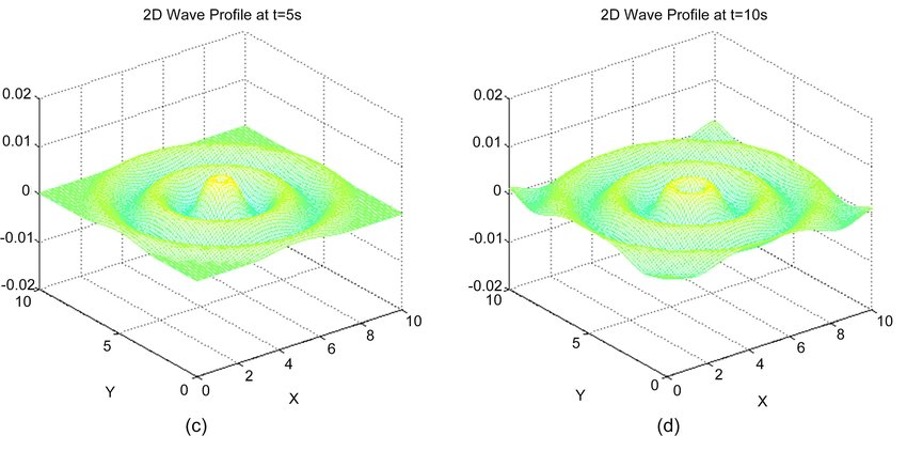
\includegraphics[width=0.7\textwidth]{ljud.png}
\caption{Visualisering av ljudvågor i två dimensioner.}
\label{fig:ljud}
\end{figure}


\clearpage
\section{2D-vågekvationen (huvudlagen)}
Utgångspunkten för modellen är vågekvationen, som beskriver hur akustiska 
tryckvågor sprids i ett homogent medium. För ett homogent medium beskrivs 
ljudutbredning i ett 2D-plan av:

\begin{equation}
\frac{\partial^2 p}{\partial t^2}
=
c^2\left(
\frac{\partial^2 p}{\partial x^2}
+
\frac{\partial^2 p}{\partial y^2}
\right)
\end{equation}

Vågekvationen beskriver hur tryckfältets tidsutveckling
bestäms av dess rumsliga variation. Krökning i tryckfältet
genererar därmed acceleration i tiden, vilket ger upphov
till vågutbredning.


\subsection{Diskretisering av vågekvationen}
För att kunna simulera vågekvationen på en dator måste den kontinuerliga
ekvationen diskretiseras. Detta innebär att rummet delas upp i ett
regelbundet rutnät och tiden utvecklas i diskreta steg.

Vi introducerar därför följande diskreta variabler:

\[
p_{i,j}^n \approx p(x_i, y_j, t_n)
\]

där $x_i = i \Delta x, \quad y_j = j \Delta x, \quad t_n = n \Delta t$. 
$\Delta x$ är den spatiala gridstorleken, $\Delta t$ tidssteget, 
$i,j$ gridindex i rummet och $n$ tidsindex.
Tryckfältet representeras alltså numeriskt som ett tvådimensionellt
fält där varje punkt uppdateras vid varje tidssteg. De partiella 
derivatorna i vågekvationen approximeras med centrala differenser.

Den andra derivatan i tiden approximeras som

\[
\frac{\partial^2 p}{\partial t^2}
\approx
\frac{p_{i,j}^{n+1} - 2p_{i,j}^{n} + p_{i,j}^{n-1}}{(\Delta t)^2}
\]

De rumsliga derivatorna approximeras som

\[
\frac{\partial^2 p}{\partial x^2}
\approx
\frac{p_{i+1,j}^n - 2p_{i,j}^n + p_{i-1,j}^n}{(\Delta x)^2}
\]

\[
\frac{\partial^2 p}{\partial y^2}
\approx
\frac{p_{i,j+1}^n - 2p_{i,j}^n + p_{i,j-1}^n}{(\Delta x)^2}
\]

Genom att ersätta derivatorna i vågekvationen med dessa
diskreta approximationer och lösa ut $p_{i,j}^{n+1}$ erhålls
den diskreta uppdateringsregeln.

Insättning av dessa approximationer i vågekvationen ger

\[
\frac{p_{i,j}^{n+1}-2p_{i,j}^{n}+p_{i,j}^{n-1}}{(\Delta t)^2}
=
c^2
\frac{
p_{i+1,j}^n+p_{i-1,j}^n+p_{i,j+1}^n+p_{i,j-1}^n-4p_{i,j}^n
}{(\Delta x)^2}
\]

vilket efter omskrivning ger den diskreta uppdateringsregeln nedan.
Denna ekvation används sedan för att beräkna hur tryckfältet
utvecklas över tid i simuleringen.

Multiplikation med $(\Delta t)^2$ ger

\[
p_{i,j}^{n+1} - 2p_{i,j}^{n} + p_{i,j}^{n-1}
=
c^2 \frac{(\Delta t)^2}{(\Delta x)^2}
\left(
p_{i+1,j}^n + p_{i-1,j}^n + p_{i,j+1}^n + p_{i,j-1}^n - 4p_{i,j}^n
\right)
\]

Genom att definiera $r = \frac{c\Delta t}{\Delta x}$ fås uppdateringsregeln nedan.


\subsection{Diskret 2D-vågekvation (numerisk modell)}
Denna metod kallas Finite Difference Time Domain (FDTD)
och är en standardmetod för att lösa vågekvationer numeriskt.

\begin{equation}
p_{i,j}^{n+1}
=
2p_{i,j}^n - p_{i,j}^{n-1}
+
r^2
\left(
p_{i+1,j}^n + p_{i-1,j}^n
+
p_{i,j+1}^n + p_{i,j-1}^n
-
4p_{i,j}^n
\right)
\end{equation}

Uttrycket inom parentes motsvarar den diskreta
Laplacianen i två dimensioner och beskriver hur
tryckfältet varierar i förhållande till sina fyra
närmaste grannar i rutnätet.

Pseudokod:
\begin{lstlisting}[style=pseudocode]
function fdtd_step_pressure(p_now, p_prev, c, dt, dx):
  # p_now  : pressure field at time step n
  # p_prev : pressure field at time step n-1
  r = (c*dt) / dx
  assert r <= 1/sqrt(2)   # CFL condition for 2D

  p_next = array_like(p_now)

  for each interior cell (i,j):
    lap =
      p_now[i+1,j] + p_now[i-1,j] +
      p_now[i,j+1] + p_now[i,j-1] -
      4*p_now[i,j]

    p_next[i,j] = 2*p_now[i,j] - p_prev[i,j] + (r*r)*lap

  apply_boundary_conditions(p_next)
  return p_next
\end{lstlisting}

\subsubsection{CFL-villkoret}

Den diskreta modellen innehåller den dimensionslösa parametern

\[
r = \frac{c\Delta t}{\Delta x}
\]

som kallas CFL-talet.
För att den numeriska lösningen ska vara stabil måste
$r \le \frac{1}{\sqrt{2}}$ gälla.
Storheten $c\Delta t$ motsvarar hur långt en våg färdas under ett
tidssteg, medan $\Delta x$ är avståndet mellan två gridpunkter.
Villkoret innebär därför att vågen inte får förflytta sig mer än
ungefär en gridcell per tidssteg.


\subsection{Superposition}
Eftersom vågekvationen är linjär gäller superpositionsprincipen:
summan av flera lösningar är också en lösning:

\begin{equation}
p_{\text{tot}}(x,y,t) = \sum_i p_i(x,y,t)
\end{equation}

Detta gör att interferens, förstärkning och utsläckning uppstår
automatiskt när flera ljudkällor bidrar samtidigt.


\clearpage
\section{Medium och material}
Utöver själva vågutbredningen påverkas ljudet även av egenskaper
hos det medium som vågen färdas genom. Dessa egenskaper avgör

\begin{itemize}
\item hur snabbt vågor sprids
\item hur mycket energi som förloras under propagation
\item hur vågor reflekteras vid gränser mellan material
\end{itemize}

I simuleringen representeras ljudet av tryckfältet $p(x,y,t)$.
Materialegenskaper påverkar därför direkt hur detta fält utvecklas
över tid i varje punkt i planet.


\subsection{Bakgrundsmedium och lokala material}
Simuleringen utgår från ett homogent bakgrundsmedium som fyller
hela planet. Detta medium är normalt luft men kan även vara
exempelvis vatten beroende på hur simuleringen initialiseras.

Bakgrundsmediet definierar de grundläggande materialparametrarna
i hela domänen, såsom ljudhastighet, densitet och dämpning.
Dessa parametrar används i varje punkt i tryckfältet
$p(x,y,t)$ så länge inget annat material är närvarande.

I spelet kan användaren placera objekt i planet, exempelvis
väggar eller hinder. Dessa objekt representerar andra material,
såsom trä, betong eller metall. När ett objekt placeras i
simuleringen överskriver dess materialparametrar de
bakgrundsparametrar som annars gäller i dessa positioner.

I den diskreta modellen delas rummet upp i ett rutnät där varje
punkt representeras av en cell $(i,j)$. Varje cell tilldelas ett
material som bestämmer vilka fysikaliska parametrar som används
i just den positionen.

\[
p_{i,j}^n \quad \rightarrow \quad \text{material}(i,j)
\]

Detta innebär att olika delar av planet kan ha olika
materialegenskaper samtidigt.

När ett objekt flyttas i spelet uppdateras materialet i de
gridceller som objektet täcker innan nästa tidssteg i
simuleringen beräknas. På så sätt kan material förändras
dynamiskt utan att själva vågekvationen behöver ändras.

Pseudokod:
\begin{lstlisting}[style=pseudocode]
function rebuild_material_field(base_material, objects):

  for each cell (i,j):
      material[i,j] = base_material

  for each object in objects:
      for each cell covered by object:
          material[i,j] = object.material
\end{lstlisting}

Själva vågsimuleringen använder sedan materialfältet för att
hämta rätt fysikaliska parametrar i varje punkt i planet.
Detta gör att olika medium kan samexistera i simuleringen
och påverka hur ljudvågor sprids och reflekteras.


\subsection{Dämpning i mediet}
När ljudvågor propagerar genom ett medium förloras en del av
vågens energi genom flera fysikaliska processer, bland annat
viskös friktion i vätskan eller gasen, värmeledning mellan 
kompression och expansion och interna rörelser i materialets 
struktur. Dessa processer gör att vågens amplitud gradvis 
minskar när vågen färdas genom mediet.


\subsubsection{Kontinuerlig modell}
I en kontinuerlig beskrivning kan denna energiförlust modelleras
som en exponentiell avklingning av amplituden

\[
p(d) = p_0 e^{-\alpha d}
\]

där $p_0$ är initial amplitud, \quad $d$ är färdad sträcka, \quad
$\alpha$ är en absorptionskoefficient som beror på materialet.

Eftersom ljudvågor färdas med hastigheten $c$ gäller sambandet
$d = ct$ vilket innebär att dämpningen även kan uttryckas som 
en funktion av tiden.


\subsubsection{Diskret implementering}
I den numeriska simuleringen representeras tryckfältet av värden
i varje punkt i rutnätet:

\[
p_{i,j}^n
\]

I stället för att beräkna exakt hur långt varje våg har färdats
modelleras energiförlusten genom en enkel tidsbaserad dämpning.
Vid varje tidssteg multipliceras tryckfältet med en faktor

\[
p_{i,j}^n \leftarrow \beta\, p_{i,j}^n
\]

där $0 < \beta < 1$ är en parameter som bestämmer hur snabbt 
amplituden avtar. Denna modell innebär att vågor som existerar 
längre tid i simuleringen gradvis förlorar energi, oberoende 
av hur de reflekteras eller interfererar i systemet.

Pseudokod:
\begin{lstlisting}[style=pseudocode]
function apply_damping(field, beta):
  for each cell (i,j):
    field[i,j] = beta * field[i,j]
\end{lstlisting}

I praktiken appliceras denna dämpning direkt på tryckfältet 
$p(x,y,t)$ och påverkar därför alla vågor i simuleringen 
oberoende av deras ursprung. FDTD-uppdateringen sker för 
varje tidssteg i tryckfältet.


\subsection{Materialparametrar}
Olika material påverkar ljudvågor genom ett antal fysikaliska
egenskaper. De viktigaste i akustik är densitet $\rho$, 
ljudhastighet $c$ och akustisk impedans $Z$.

Dessa storheter bestämmer både hur snabbt vågor sprids i
materialet och hur vågor beter sig vid gränser mellan
olika material.


\subsubsection{Ljudhastighet}
Ljudhastigheten bestämmer hur snabbt tryckvariationer
sprids genom mediet. Den beror på materialets elasticitet
och densitet. För en ideal gas ges ljudhastigheten av:

\begin{equation}
c = \sqrt{\gamma \frac{RT}{M}}
\end{equation}

I praktiska simuleringar används ofta en enklare
approximation för luft

\begin{equation}
c(T) \approx 331 + 0.6T
\end{equation}

där $T$ är temperaturen i $^\circ$C och $c$ erhålls i m/s.

Pseudokod:
\begin{lstlisting}[style=pseudocode]
function speed_of_sound_air(T_celsius):
  return 331 + 0.6*T_celsius
\end{lstlisting}

Genom att ändra värdet på $c$ kan simuleringen enkelt
representera olika medium såsom luft, vatten eller fasta
material.


\subsubsection{Akustisk impedans}
Den akustiska impedansen definieras som

\begin{equation}
Z = \rho c
\end{equation}

Impedansen beskriver hur svårt det är för en ljudvåg
att sätta materialet i rörelse. Den spelar en central
roll när en våg möter en gräns mellan två material.

Pseudokod:
\begin{lstlisting}[style=pseudocode]
function impedance(rho, c):
  assert rho > 0 and c > 0
  return rho * c
\end{lstlisting}


\subsection{Reflektion och transmission}
När en ljudvåg når en gräns mellan två material med olika
akustisk impedans delas vågen upp i två komponenter:

\begin{itemize}
\item en reflekterad våg som fortsätter i det första materialet
\item en transmitterad våg som fortsätter in i det andra materialet
\end{itemize}

Vid normal infallsvinkel ges amplitudkoefficienterna av
\begin{align}
R &= \frac{Z_2 - Z_1}{Z_2 + Z_1} \\
T &= \frac{2Z_2}{Z_2 + Z_1}
\end{align}

där $Z_1$ och $Z_2$ är impedanserna i de två materialen.

Reflektionskoefficienten $R$ anger hur stor del av
vågens amplitud som reflekteras, medan
transmissionskoefficienten $T$ anger hur stor del
som fortsätter in i det andra materialet.
Den reflekterade energin är proportionell mot $|R|^2$.

Pseudokod:
\begin{lstlisting}[style=pseudocode]
function reflection_coeff(Z1, Z2):
  denom = Z1 + Z2
  assert denom != 0
  return (Z2 - Z1) / denom

function transmission_coeff(Z1, Z2):
  denom = Z1 + Z2
  assert denom != 0
  return (2*Z2) / denom
\end{lstlisting}

I den tvådimensionella simuleringen innebär detta att
när en vågfront i tryckfältet $p(x,y,t)$ når en gräns
mellan två material kommer en del av vågen att studsa
tillbaka medan resten fortsätter in i det nya materialet.
Skillnader i impedans avgör hur stark denna reflektion
blir.

\clearpage
\section{Piano som källa}
\subsection{Tangent $\rightarrow$ frekvens (liksvävig temperatur)}
\begin{equation}
f_n = 440 \cdot 2^{n/12}
\end{equation}
där $n=0$ motsvarar A4 (440 Hz).

Pseudokod:
\begin{lstlisting}[style=pseudocode]
function piano_frequency(semitones_from_A4):
  return 440 * 2^(semitones_from_A4/12)
\end{lstlisting}

Liksvävig temperatur innebär att varje halvton är separerad
av en konstant frekvensfaktor $2^{1/12}$.
Detta möjliggör spel i alla tonarter utan omstämning.
Som visas i Figur \ref{fig:piano} representeras olika noter 
med olika frekvenser.

\begin{figure}[h]
\centering
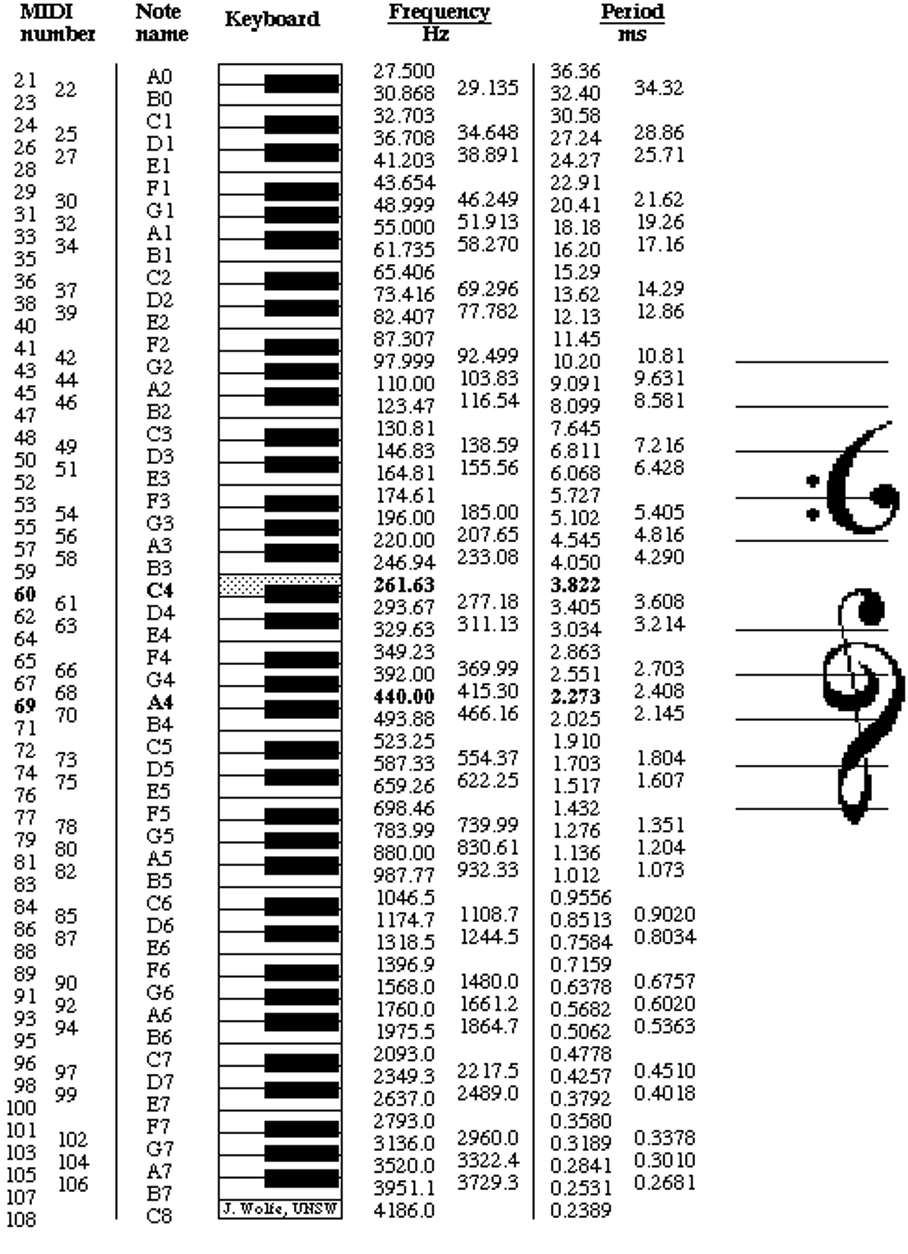
\includegraphics[width=0.6\textwidth]{piano.png}
\caption{Piano som ljudkälla i modellen.}
\label{fig:piano}
\end{figure}

\clearpage
\subsection{Harmonisk serie och signalmodell}
\begin{equation}
f_n = n f_1
\end{equation}

Pseudokod:
\begin{lstlisting}[style=pseudocode]
function harmonic_frequency(n, f1):
  assert n >= 1
  return n * f1
\end{lstlisting}

En förenklad modell för tonens trycksignal:
\begin{equation}
p(t) = \sum_{n=1}^N A_n \cos(2\pi n f_1 t + \phi_n)
\end{equation}

Pseudokod:
\begin{lstlisting}[style=pseudocode]
function piano_signal(t, f1, A, phi, N):
  # A[k], phi[k] for k=1..N
  sum = 0
  for k in 1..N:
    sum += A[k] * cos(2*pi*k*f1*t + phi[k])
  return sum
\end{lstlisting}

En pianoton består inte av en enda frekvens utan av flera
harmoniska övertoner.
Det är summan av dessa komponenter som ger instrumentet
dess karakteristiska klang.
När strängen vibrerar sätter den i sin tur ljudbrädan i rörelse,
vilket kopplar strängens mekaniska vibration till luftens tryckfält.
Det är denna koppling som genererar den akustiska tryckvågen
som sedan beskrivs av 2D-vågekvationen i simuleringen.
I modellen representeras denna process genom att pianotonen
introduceras som en tryckkälla i planet.
Detta tryckbidrag adderas till tryckfältet p(x,y,t) i
simuleringen och utvecklas därefter enligt vågekvationen.

\end{document}